\subsection{Wavelength Wonders: The Length of a 14.10 MHz Transmission Line!}

\begin{tcolorbox}[colback=gray!10, colframe=black, title=E9F06] What is the approximate physical length of an air-insulated, parallel conductor transmission line that is electrically 1/2 wavelength long at 14.10 MHz?

\begin{enumerate}[label=\Alph*.]
    \item 7.0 meters
    \item 8.5 meters
    \item \textbf{10.6 meters}
    \item 13.3 meters
\end{enumerate} \end{tcolorbox}

\subsubsection{Concepts Required}

To answer this question, we need to understand the relationship between the frequency of a signal and its wavelength. The wavelength (\(\lambda\)) of a radio wave can be calculated using the formula:

\[
\lambda = \frac{c}{f}
\]

where:
- \(c\) is the speed of light in a vacuum, approximately \(3 \times 10^8\) meters per second,
- \(f\) is the frequency in hertz (Hz).

In this case, the frequency \(f\) is \(14.10\) MHz, which we convert into hertz:

\[
f = 14.10 \times 10^6 \text{ Hz}
\]

Now, we can substitute this value into the wavelength equation:

\[
\lambda = \frac{3 \times 10^8 \text{ m/s}}{14.10 \times 10^6 \text{ Hz}}
\]

Calculating the wavelength:

\[
\lambda = \frac{3 \times 10^8}{14.10 \times 10^6} \approx 21.3 \text{ meters}
\]

Since the question asks for the length of a transmission line that is electrically 1/2 wavelength long, we must divide the calculated wavelength by 2:

\[
\text{Length} = \frac{\lambda}{2} = \frac{21.3 \text{ meters}}{2} \approx 10.65 \text{ meters}
\]

Thus, the approximate physical length of the transmission line is about \(10.65\) meters, which rounds to approximately \(10.6\) meters.

\subsubsection{Conclusion}

The correct answer to the question is choice C: \textbf{10.6 meters}. Understanding the relationship between frequency and wavelength is crucial in fields such as radio communication and electronics.

\subsubsection{Diagram}

\begin{center}
    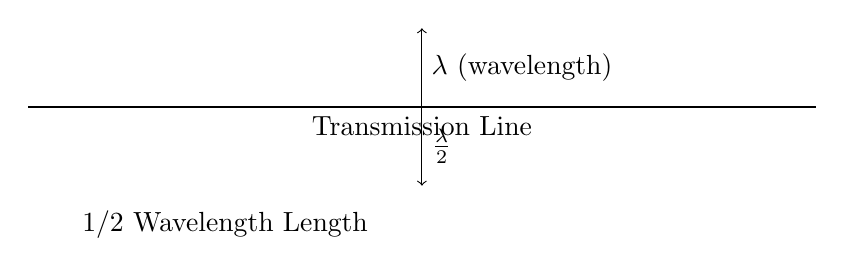
\begin{tikzpicture}
        \draw [-] (0,0) -- (10,0) node[midway, below] {Transmission Line};
        \draw[->] (5, 0) -- (5, 1) node[midway,right] {$\lambda$ (wavelength)};
        \draw[->] (5,0) -- (5,-1) node[midway,right] {$\frac{\lambda}{2}$};
        \draw (2.5,-1.5) node {1/2 Wavelength Length};
    \end{tikzpicture}
\end{center}
